% Four representations through a reference resolver, with a DataLoader behind
% it and without one. Referenced from chapter 11. Bare tikzpicture; the figure
% environment, caption and label live at the call site.
%
% The point of the picture is that the left column has one lookup and the right
% column has four, and that the reason is not the number of calls: both columns
% enter the resolver four times. What differs is whether the four calls are in
% flight at the same moment.
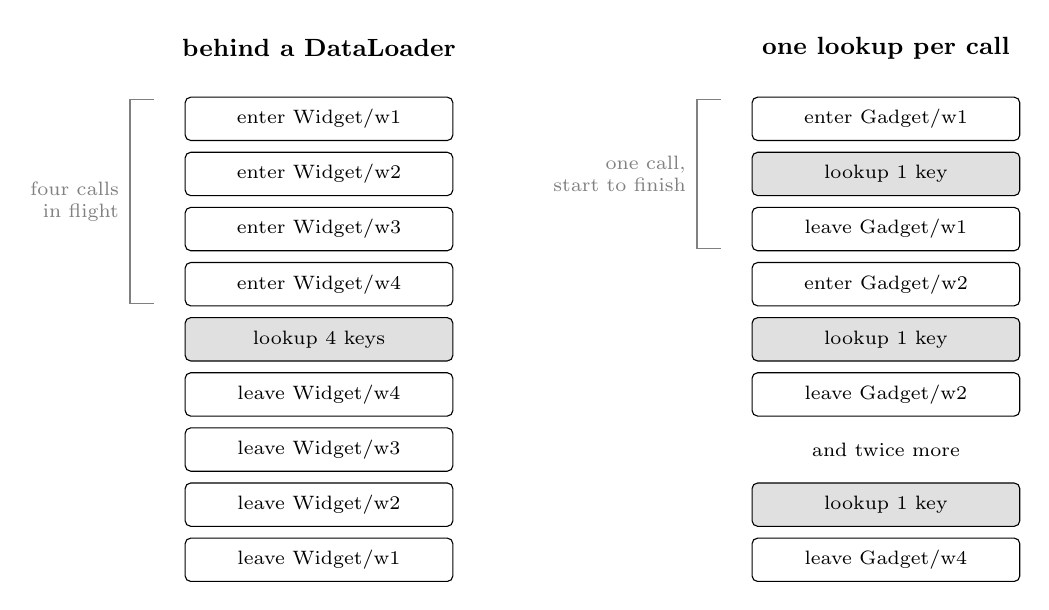
\begin{tikzpicture}[
    font=\small,
    head/.style={font=\small\bfseries, align=center},
    call/.style={draw, rounded corners=2pt, minimum width=34mm,
                 minimum height=5.5mm, align=center, font=\scriptsize},
    hit/.style={draw, rounded corners=2pt, minimum width=34mm,
                minimum height=5.5mm, align=center, font=\scriptsize,
                fill=black!12},
    span/.style={gray},
    lbl/.style={font=\scriptsize, align=center, inner sep=1pt}
  ]

  \node[head] at (2.6,0.6)  {behind a DataLoader};
  \node[head] at (9.8,0.6)  {one lookup per call};

  % -- left column: all four enter, then one lookup --------------------------
  \node[call] (l1) at (2.6,-0.3) {\code{enter  Widget/w1}};
  \node[call] (l2) at (2.6,-1.0) {\code{enter  Widget/w2}};
  \node[call] (l3) at (2.6,-1.7) {\code{enter  Widget/w3}};
  \node[call] (l4) at (2.6,-2.4) {\code{enter  Widget/w4}};
  \node[hit]  (lb) at (2.6,-3.1) {\code{lookup 4 keys}};
  \node[call] (l5) at (2.6,-3.8) {\code{leave  Widget/w4}};
  \node[call] (l6) at (2.6,-4.5) {\code{leave  Widget/w3}};
  \node[call] (l7) at (2.6,-5.2) {\code{leave  Widget/w2}};
  \node[call] (l8) at (2.6,-5.9) {\code{leave  Widget/w1}};

  \draw[span] (0.5,-0.05) -- (0.2,-0.05) -- (0.2,-2.65) -- (0.5,-2.65);
  \node[lbl, span, anchor=east, align=right] at (0.1,-1.35)
    {four calls\\in flight};

  % -- right column: enter, lookup, leave, four times ------------------------
  \node[call] (r1) at (9.8,-0.3) {\code{enter  Gadget/w1}};
  \node[hit]  (r2) at (9.8,-1.0) {\code{lookup 1 key}};
  \node[call] (r3) at (9.8,-1.7) {\code{leave  Gadget/w1}};
  \node[call] (r4) at (9.8,-2.4) {\code{enter  Gadget/w2}};
  \node[hit]  (r5) at (9.8,-3.1) {\code{lookup 1 key}};
  \node[call] (r6) at (9.8,-3.8) {\code{leave  Gadget/w2}};
  \node[lbl]        at (9.8,-4.5) {and twice more};
  \node[hit]  (r7) at (9.8,-5.2) {\code{lookup 1 key}};
  \node[call] (r8) at (9.8,-5.9) {\code{leave  Gadget/w4}};

  \draw[span] (7.7,-0.05) -- (7.4,-0.05) -- (7.4,-1.95) -- (7.7,-1.95);
  \node[lbl, span, anchor=east, align=right] at (7.3,-1.0)
    {one call,\\start to finish};

\end{tikzpicture}
